%&"../main"
\documentclass[../main]{subfiles}
\begin{document}

\chapter{融资分析}%
\label{cha:融资分析}

\section{资产负债率}%
\label{sec:资产负债率}

首先,从华为负债融资现状来看,近几年华为资产负债率在不断提高,如果跨国公司的资产
负债率达到7\%,则公司将无法再进行外部债务融资。由此可见,华为公司资产 负债率已经
逼近跨国公司债务融资比例上限,这无疑会为 华为后期融资产生不利影响,而融资受阻自
然也会影响到 华为公司跨国经营的正常发展和业务扩张。

\begin{figure}[htbp]
	\centering
	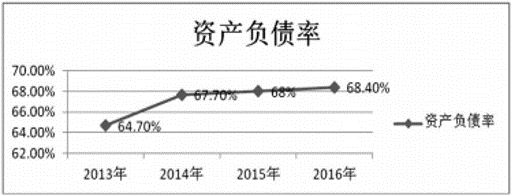
\includegraphics[width = 0.8\linewidth]{capital.png}
	\caption{资产负债率}
	\label{fig:资产负债率}
\end{figure}

\section{融资结构}%
\label{sec:融资结构}

从债务融资的规模和构成来看,华为公司2014~2016年的债务融资总规模在不断扩大,债务
规模短期内大幅提高,而公司短期借款保持稳定。此外,在债务融资的流动性方面,华为通
过大幅调整非流动性负债而降低流动性负债来减轻公司短期偿债压力,增强公司财务稳定性
和资金充足性。综上,华为公司近几年通过多元化的融资渠道,大规模提高了债务融资规模
,而在债务融资选择方式上,华为选择增加长期负债和非流动性负债,保持短期负债并降低
流动性负债的方式以调整自身债务融资结构,既为自身跨国经营提供充足的资金支持,也能
有效控制自身财务风险。

\begin{figure}[htbp]
	\centering
	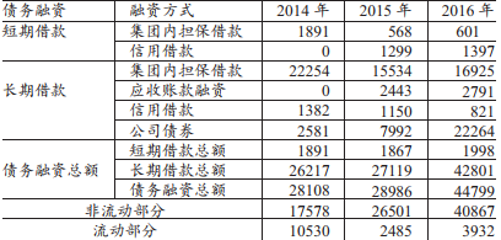
\includegraphics[width = 0.8\linewidth]{construction.png}
	\caption{融资结构}
	\label{fig:融资结构}
\end{figure}

债务融资的成本上看,华为选择了扩大集团 内部担保借款和发行企业债券占比,而在融资
的币种选择方面华为主要选择了欧元、美元和人民币。在融资利率类型选择方面,华为倾向
于短期负债选择浮动利率;长期负债倾向于选择固定利率的模式,也倾向于以美元作为结算
货币发行债券,。综上所述,华为在控制债务融资成本方面,选择扩大以美元作为结算货币
进行短期和长期融资比例,因为美元作为国际货币便于跨国经营过程中资金结算的同时也能
有效抵消人民币对美元汇率变动产生的汇兑损失,进而更有利于从总体上控制企业债务融资
成本总额。

\begin{figure}[htbp]
	\centering
	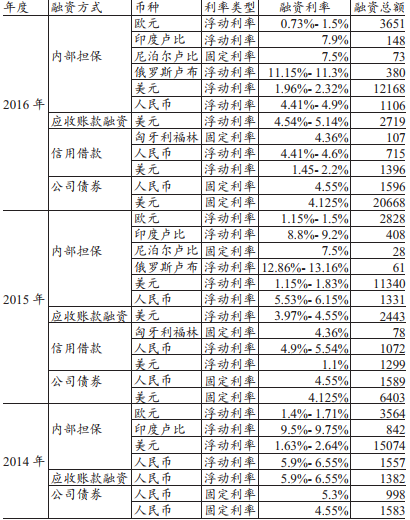
\includegraphics[width = 0.8\linewidth]{time.png}
	\caption{融资方式}
	\label{fig:融资方式}
\end{figure}

\section{优化建议}%
\label{sec:优化建议}

\begin{description}

	\item[保持合理的债务融资比重]跨国公司应综合考虑影响债务水平的因素,采取
		一个合理的债务融资比重。考虑这一比重的因素包括产业的多元化经营、
		东道国的税收政策和金融市场发展水平、企业的国际化水平、代理成本、
		汇率风险等。不能为了获得更高的避税收益而采取过高的债务融资,也不
		能过于担心陷入财务困境而采取过低的债务融资。一般而言,当跨国公司
		的国际化水平较高时,可以采取相对较高的债务融资比重,如华为的债务
		融资比重基本大于60\%,这与其较高的国际化程度是相符的。;

	\item[建立多元的债务融资结构]东道国的金融发展水平对跨国公司债务融资具有
		正向的效应。若跨国公司在发达国家东道国中自然能进入到更发达的金融
		资本市场中,从而以成本更低的融资方式进行债券融资,使其融资结构更
		为多元。华为就采取了包括公司债券和银行组团贷款等多种债务融资方式
		。为了达到规避资金供应潜在风险,同时降低债务融资成本、优化债务融
		资结构的目的,跨国公司应当借助跨国经营的模式,利用发达国家东道国
		的发达金融资本市场,进行多渠道、多元化的融资资源拓展与融资结构管
		理。;

	\item[增加境外融资的比重]东道国的税收政策对跨国公司债务融资具有影响,高
		于母国的东道国税率有助于使债务融资产生更多的避税收益,因此跨国公
		司可以通过在母子公司之间调整债务融资比例,最大化避税收益。华为即
		是充分利用了境外融资的优势,境外融资的比重较高,优化自己的债务融
		资结构,使其即满足了流动资金需求,又实现了低成本利用境外资本的可
		能。跨国公司应当审时度势,适当增加境外融资的比重,建立适合本公司
		的最优融资结构。

\end{description}

\end{document}

